% Options for packages loaded elsewhere
\PassOptionsToPackage{unicode}{hyperref}
\PassOptionsToPackage{hyphens}{url}
%
\documentclass[
]{article}
\usepackage{amsmath,amssymb}
\usepackage{iftex}
\ifPDFTeX
  \usepackage[T1]{fontenc}
  \usepackage[utf8]{inputenc}
  \usepackage{textcomp} % provide euro and other symbols
\else % if luatex or xetex
  \usepackage{unicode-math} % this also loads fontspec
  \defaultfontfeatures{Scale=MatchLowercase}
  \defaultfontfeatures[\rmfamily]{Ligatures=TeX,Scale=1}
\fi
\usepackage{lmodern}
\ifPDFTeX\else
  % xetex/luatex font selection
\fi
% Use upquote if available, for straight quotes in verbatim environments
\IfFileExists{upquote.sty}{\usepackage{upquote}}{}
\IfFileExists{microtype.sty}{% use microtype if available
  \usepackage[]{microtype}
  \UseMicrotypeSet[protrusion]{basicmath} % disable protrusion for tt fonts
}{}
\makeatletter
\@ifundefined{KOMAClassName}{% if non-KOMA class
  \IfFileExists{parskip.sty}{%
    \usepackage{parskip}
  }{% else
    \setlength{\parindent}{0pt}
    \setlength{\parskip}{6pt plus 2pt minus 1pt}}
}{% if KOMA class
  \KOMAoptions{parskip=half}}
\makeatother
\usepackage{xcolor}
\usepackage[margin=1in]{geometry}
\usepackage{color}
\usepackage{fancyvrb}
\newcommand{\VerbBar}{|}
\newcommand{\VERB}{\Verb[commandchars=\\\{\}]}
\DefineVerbatimEnvironment{Highlighting}{Verbatim}{commandchars=\\\{\}}
% Add ',fontsize=\small' for more characters per line
\usepackage{framed}
\definecolor{shadecolor}{RGB}{248,248,248}
\newenvironment{Shaded}{\begin{snugshade}}{\end{snugshade}}
\newcommand{\AlertTok}[1]{\textcolor[rgb]{0.94,0.16,0.16}{#1}}
\newcommand{\AnnotationTok}[1]{\textcolor[rgb]{0.56,0.35,0.01}{\textbf{\textit{#1}}}}
\newcommand{\AttributeTok}[1]{\textcolor[rgb]{0.13,0.29,0.53}{#1}}
\newcommand{\BaseNTok}[1]{\textcolor[rgb]{0.00,0.00,0.81}{#1}}
\newcommand{\BuiltInTok}[1]{#1}
\newcommand{\CharTok}[1]{\textcolor[rgb]{0.31,0.60,0.02}{#1}}
\newcommand{\CommentTok}[1]{\textcolor[rgb]{0.56,0.35,0.01}{\textit{#1}}}
\newcommand{\CommentVarTok}[1]{\textcolor[rgb]{0.56,0.35,0.01}{\textbf{\textit{#1}}}}
\newcommand{\ConstantTok}[1]{\textcolor[rgb]{0.56,0.35,0.01}{#1}}
\newcommand{\ControlFlowTok}[1]{\textcolor[rgb]{0.13,0.29,0.53}{\textbf{#1}}}
\newcommand{\DataTypeTok}[1]{\textcolor[rgb]{0.13,0.29,0.53}{#1}}
\newcommand{\DecValTok}[1]{\textcolor[rgb]{0.00,0.00,0.81}{#1}}
\newcommand{\DocumentationTok}[1]{\textcolor[rgb]{0.56,0.35,0.01}{\textbf{\textit{#1}}}}
\newcommand{\ErrorTok}[1]{\textcolor[rgb]{0.64,0.00,0.00}{\textbf{#1}}}
\newcommand{\ExtensionTok}[1]{#1}
\newcommand{\FloatTok}[1]{\textcolor[rgb]{0.00,0.00,0.81}{#1}}
\newcommand{\FunctionTok}[1]{\textcolor[rgb]{0.13,0.29,0.53}{\textbf{#1}}}
\newcommand{\ImportTok}[1]{#1}
\newcommand{\InformationTok}[1]{\textcolor[rgb]{0.56,0.35,0.01}{\textbf{\textit{#1}}}}
\newcommand{\KeywordTok}[1]{\textcolor[rgb]{0.13,0.29,0.53}{\textbf{#1}}}
\newcommand{\NormalTok}[1]{#1}
\newcommand{\OperatorTok}[1]{\textcolor[rgb]{0.81,0.36,0.00}{\textbf{#1}}}
\newcommand{\OtherTok}[1]{\textcolor[rgb]{0.56,0.35,0.01}{#1}}
\newcommand{\PreprocessorTok}[1]{\textcolor[rgb]{0.56,0.35,0.01}{\textit{#1}}}
\newcommand{\RegionMarkerTok}[1]{#1}
\newcommand{\SpecialCharTok}[1]{\textcolor[rgb]{0.81,0.36,0.00}{\textbf{#1}}}
\newcommand{\SpecialStringTok}[1]{\textcolor[rgb]{0.31,0.60,0.02}{#1}}
\newcommand{\StringTok}[1]{\textcolor[rgb]{0.31,0.60,0.02}{#1}}
\newcommand{\VariableTok}[1]{\textcolor[rgb]{0.00,0.00,0.00}{#1}}
\newcommand{\VerbatimStringTok}[1]{\textcolor[rgb]{0.31,0.60,0.02}{#1}}
\newcommand{\WarningTok}[1]{\textcolor[rgb]{0.56,0.35,0.01}{\textbf{\textit{#1}}}}
\usepackage{longtable,booktabs,array}
\usepackage{calc} % for calculating minipage widths
% Correct order of tables after \paragraph or \subparagraph
\usepackage{etoolbox}
\makeatletter
\patchcmd\longtable{\par}{\if@noskipsec\mbox{}\fi\par}{}{}
\makeatother
% Allow footnotes in longtable head/foot
\IfFileExists{footnotehyper.sty}{\usepackage{footnotehyper}}{\usepackage{footnote}}
\makesavenoteenv{longtable}
\usepackage{graphicx}
\makeatletter
\def\maxwidth{\ifdim\Gin@nat@width>\linewidth\linewidth\else\Gin@nat@width\fi}
\def\maxheight{\ifdim\Gin@nat@height>\textheight\textheight\else\Gin@nat@height\fi}
\makeatother
% Scale images if necessary, so that they will not overflow the page
% margins by default, and it is still possible to overwrite the defaults
% using explicit options in \includegraphics[width, height, ...]{}
\setkeys{Gin}{width=\maxwidth,height=\maxheight,keepaspectratio}
% Set default figure placement to htbp
\makeatletter
\def\fps@figure{htbp}
\makeatother
\ifLuaTeX
  \usepackage{luacolor}
  \usepackage[soul]{lua-ul}
\else
  \usepackage{soul}
\fi
\setlength{\emergencystretch}{3em} % prevent overfull lines
\providecommand{\tightlist}{%
  \setlength{\itemsep}{0pt}\setlength{\parskip}{0pt}}
\setcounter{secnumdepth}{-\maxdimen} % remove section numbering
\ifLuaTeX
  \usepackage{selnolig}  % disable illegal ligatures
\fi
\usepackage{bookmark}
\IfFileExists{xurl.sty}{\usepackage{xurl}}{} % add URL line breaks if available
\urlstyle{same}
\hypersetup{
  pdftitle={Aula 1 - Gabarito},
  pdfauthor={Calvin Rodrigues},
  hidelinks,
  pdfcreator={LaTeX via pandoc}}

\title{Aula 1 - Gabarito}
\author{Calvin Rodrigues}
\date{19/07/2021}

\begin{document}
\maketitle

\section{Corpo de texto}\label{corpo-de-texto}

Este é o corpo de texto do título 1

\subsection{Ênfase}\label{uxeanfase}

Para ênfase temos:

\texttt{*Itálico*\ ou\ \_Itálico\_}: \emph{Itálico}\\
\texttt{**Negrito**\ ou\ \_\_Negrito\_\_}: \textbf{Negrito}\\
\texttt{\textasciitilde{}\textasciitilde{}Tachado\textasciitilde{}\textasciitilde{}}:
\st{Tachado}

\subsection{Subscrito e sobrescrito}\label{subscrito-e-sobrescrito}

Utilizamos \texttt{\^{}sobrescrito\^{}} para sobrescrever:
2\textsuperscript{2} = 4

E utilizamos \texttt{\textasciitilde{}subscrito\textasciitilde{}} para
subscrever: a fórmula da água é H\textsubscript{2}O

\section{Links e imagens}\label{links-e-imagens}

Links e imagens têm formatação próximas

\subsection{Links}\label{links}

Há dois tipos de linkagem em R Markdown, texto âncora e links diretos

\subsubsection{Texto âncora (link em
texto)}\label{texto-uxe2ncora-link-em-texto}

Utilizamos a seguinte formatação: \texttt{{[}Texto{]}(Link)}:
\href{https://www.sympla.com.br/minicurso-elaboracao-de-relatorios-tecnicos-e-paginas-web-usando-r-markdown__1274462}{Minicurso}

\subsubsection{Link direto}\label{link-direto}

Colocamos o endereço dentro de \texttt{\textless{}Link\textgreater{}}:\\
\url{https://www.sympla.com.br/minicurso-elaboracao-de-relatorios-tecnicos-e-paginas-web-usando-r-markdown__1274462}

\subsection{Imagens}\label{imagens}

Semelhante ao código dos links porém adicionamos um \emph{!} no início

\texttt{!{[}Título\ ou\ legenda\ da\ imagem{]}(Endereço\ da\ imagem)}

\begin{figure}
\centering
\includegraphics{C:/Users/Calvin/Documents/UFJF/Curso R Markdown/minicurso.png}
\caption{Banner Minicurso}
\end{figure}

\section{Lista de itens}\label{lista-de-itens}

Para tópicos ou lista de itens utilizamos \texttt{*}, \texttt{-} ou
\texttt{+} na frente do item:

\begin{itemize}
\tightlist
\item
  Item 1
\item
  Item 2
\item
  Item 3

  \begin{itemize}
  \tightlist
  \item
    Item 3.1
  \item
    Item 3.2
  \end{itemize}
\end{itemize}

\section{Tabulação}\label{tabulauxe7uxe3o}

Para as tabelas, temos \texttt{\textbar{}} para delimitar as colunas e
\texttt{-} para delimitar os títulos, para especificar o tipo de
alinhamento usamos \texttt{:} no campo dos hífens (o padrão é
alinhamento na esquerda)

\begin{longtable}[]{@{}lcr@{}}
\toprule\noalign{}
ID & Produto & Valor \\
\midrule\noalign{}
\endhead
\bottomrule\noalign{}
\endlastfoot
01 & Computador & R\$ 3.000,00 \\
02 & Mouse & R\$ 100,00 \\
03 & Teclado & R\$ 150,00 \\
\end{longtable}

\section{Códigos}\label{cuxf3digos}

\begin{itemize}
\tightlist
\item
  Códigos inline
\item
  Múltiplas linhas de código
\end{itemize}

\begin{Shaded}
\begin{Highlighting}[]
\NormalTok{alfa }\OtherTok{=} \FunctionTok{runif}\NormalTok{ (}\DecValTok{1}\NormalTok{)}

\FunctionTok{head}\NormalTok{ (iris)}
\end{Highlighting}
\end{Shaded}

\begin{verbatim}
##   Sepal.Length Sepal.Width Petal.Length Petal.Width Species
## 1          5.1         3.5          1.4         0.2  setosa
## 2          4.9         3.0          1.4         0.2  setosa
## 3          4.7         3.2          1.3         0.2  setosa
## 4          4.6         3.1          1.5         0.2  setosa
## 5          5.0         3.6          1.4         0.2  setosa
## 6          5.4         3.9          1.7         0.4  setosa
\end{verbatim}

\begin{Shaded}
\begin{Highlighting}[]
\FunctionTok{plot}\NormalTok{ (iris}\SpecialCharTok{$}\NormalTok{Petal.Length }\SpecialCharTok{\textasciitilde{}}\NormalTok{ iris}\SpecialCharTok{$}\NormalTok{Species)}
\end{Highlighting}
\end{Shaded}

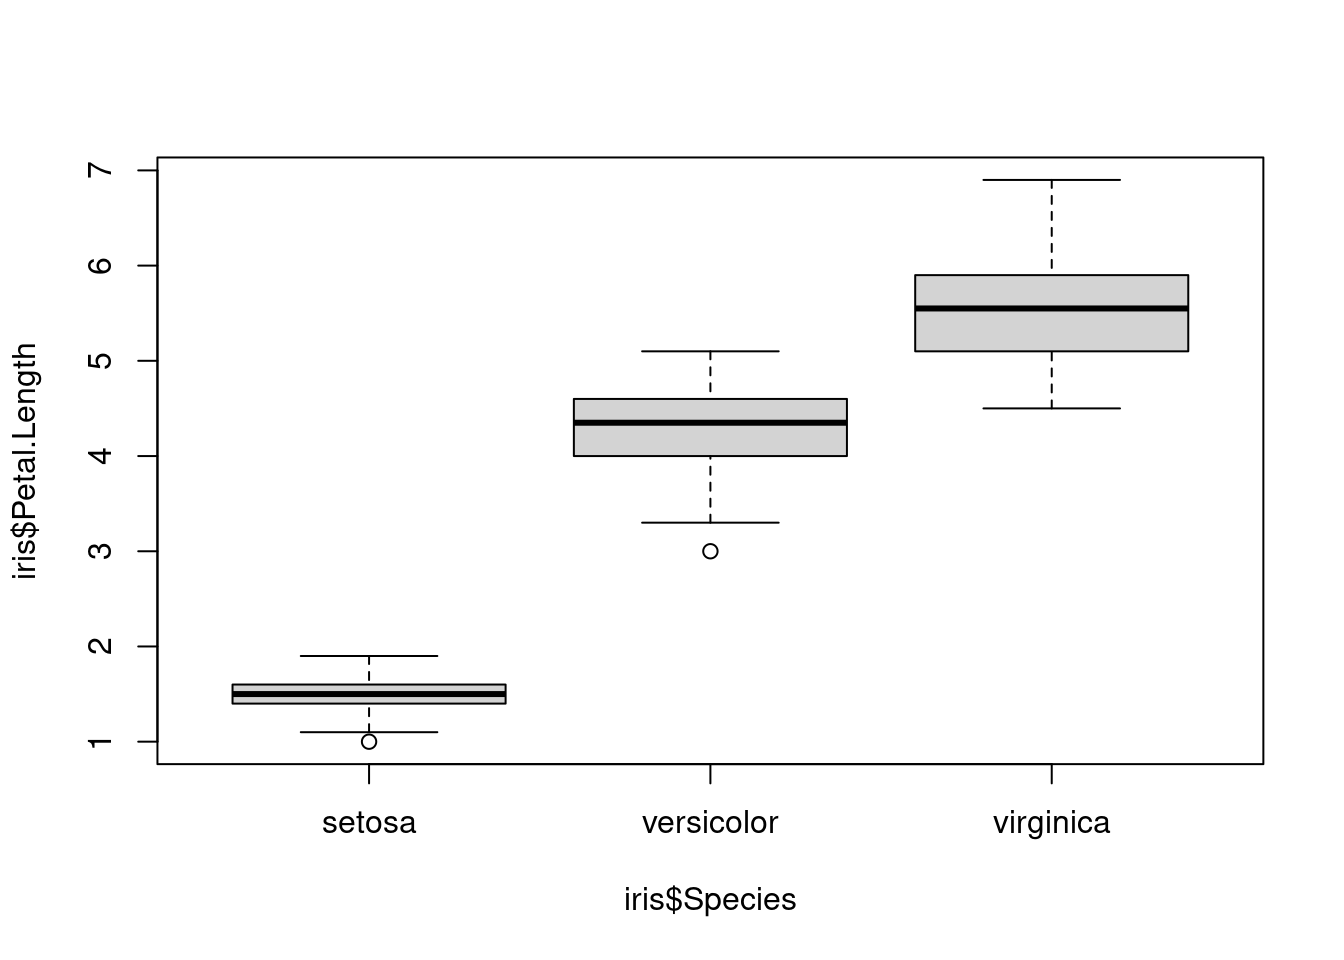
\includegraphics{Aula1Gabarito_files/figure-latex/unnamed-chunk-1-1.pdf}

O valor de alfa, que é gerado através de uma uniforme (0,1), é 0.4991414
e seu quadrado é 0.2491421

A média do comprimento das pétalas das flores é 3.758cm

\subsubsection{Parâmetros para chunk}\label{paruxe2metros-para-chunk}

\begin{itemize}
\tightlist
\item
  include
\end{itemize}

Valores são computados porém não temos a saída (output) nem o
\emph{chunk} mostrado no relatório.

O valor de alfa2, que é gerado através de uma uniforme (0,1), é
0.1345288

\begin{itemize}
\tightlist
\item
  eval
\end{itemize}

Valores não são computados e não temos a saída, porém o \emph{chunk} é
mostrado no relatório.

\begin{Shaded}
\begin{Highlighting}[]
\NormalTok{alfa3 }\OtherTok{=} \FunctionTok{runif}\NormalTok{(}\DecValTok{1}\NormalTok{)}

\FunctionTok{print}\NormalTok{ (alfa3)}
\NormalTok{alfa3}\SpecialCharTok{\^{}}\DecValTok{2}
\FunctionTok{plot}\NormalTok{ (iris}\SpecialCharTok{$}\NormalTok{Petal.Length }\SpecialCharTok{\textasciitilde{}}\NormalTok{ iris}\SpecialCharTok{$}\NormalTok{Species)}
\end{Highlighting}
\end{Shaded}

O valor de alfa3 não foi computado

\begin{itemize}
\tightlist
\item
  echo
\end{itemize}

O contrário direto do \emph{eval = FALSE}, os valores são computados e
temos a saída, porém o \emph{chunk} não é mostrado no relatório.

\begin{verbatim}
## [1] 0.2763182
\end{verbatim}

\begin{verbatim}
## [1] 0.07635176
\end{verbatim}

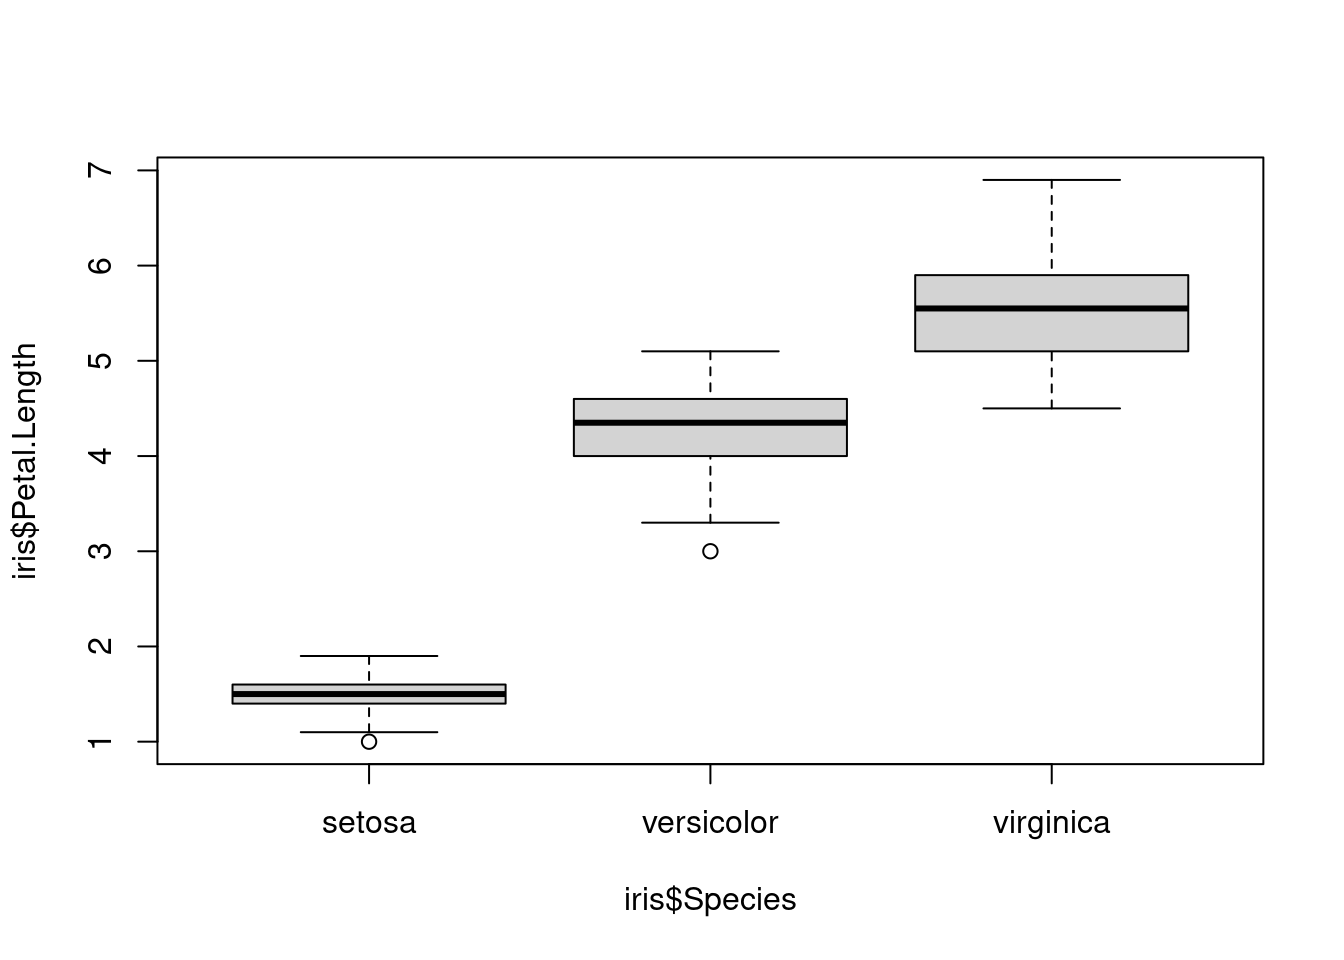
\includegraphics{Aula1Gabarito_files/figure-latex/unnamed-chunk-4-1.pdf}

O valor de alfa4, que é gerado através de uma uniforme (0,1), é
0.2763182

\end{document}
